\chapter{Evaluación experimental}
\label{cap:evaluacionexperimental}

Se utilizará predictor de tiempo para setear threads en bloques


Se hace una introducción.

\section{Predicción de tiempo de respuesta a transacción de lectura}
\label{evaluacionexperimental:ptrq}
Se hace experimentos con predictor perfecto

Nosotros optamos por un enfoque de Wand Heap Compartido para ser usado en los experimentos.

Se hace una breve introducción al cpaítulo anterior. 

Se menciona los resultados obtenidos con la regresión, se dice que no se tuvieron muy buenos resultados con la regresión, se deja a ver por qué no se obtuvieron muy buenos resultados (índice con los que se hicieron experimentos, consultas, etc.).

	//menos que 10% tpo esperado, menos que 25%, menos que 50% y el resto (en el timesRanges)
\subsection{Predictor perfecto}
\label{evaluacionexperimental:predictorperfecto}

Decir que no es el foco de esta tesi, que los resultados obtenidos no fueron muy buenos s y que para evaluar los algoritmos de scheduling  también se usará un predictor perfecto. Decir cómo se obtuvo un predictor perfecto y ojalá mostrar algún algoritmo.


\section{Wand multithreaded}
\label{evaluacionexperimental:wm}
En esta sección se muestra la implementación de las dos alternativas que se tienen para el procesamiento de consultas a través del algoritmo Wand \citep{Broder:2003}. En las secciones \ref{scheduling:wlh} y \ref{scheduling:wsh} se explica el diseño que se llevará a cabo. 

// Cómo se llevaron a cabo los experimentos
// Datos
// Máquina
// Programación 


\subsection{Wand heap local}
\label{evaluacionexperimental:wlh}
Recordar que en el esquema Wand LH cada uno de los hilos de ejecución computa el conjunto top-K local y luego la hebra maestra hace la mezcla de resultados escogiendo el mejor conjunto top-K global. Este enfoque tiene la ventaja de que es simple de implementar, puesto que no se requiere mecanismos para controlar el paralelismo entre los threads. Sin embargo, se requiere que cada uno de los (P - 1) threads envíe su conjunto solución a la hebra maestra (que también computó su propio conjunto solución), para que crear el resultado final de entre los P x K documentos, donde P es el número de threads encargadas de resolver la consulta y K se es el tamaño del conjunto que se quiere obtener. 

Los resultados en \citep{Rojas:2013} muestran indicios que el esquema LH tendría ventajas por sobre el SH para aquellas transacciones que toman poco tiempo en ser resueltas. 

El Código \ref{code:topkmultithreadwandoperatorlocal} muestra la implementación de la clase que está encargada de llevar a cabo la lógica en la ejecución del enfoque Wand LH. El método execute es el encargado de llegar a cabo la resolución de la consulta, recibe como entrada la query a ser resuelta y un vector de resultados; adicionalmente, este método es el encargado de lanzar los threads con que se resolverá cada consulta y a cada uno de ellos le asiga un objeto de tipo TopKWandOperator (arrops), para obtener los resultados y escribirlos en el vector results. Todo este proceso es llevado a cabo usando el tamaño del conjunto que se quiere obtener (k) y además el índice invertido (indice).


\begin{figure}[!th]
\centering
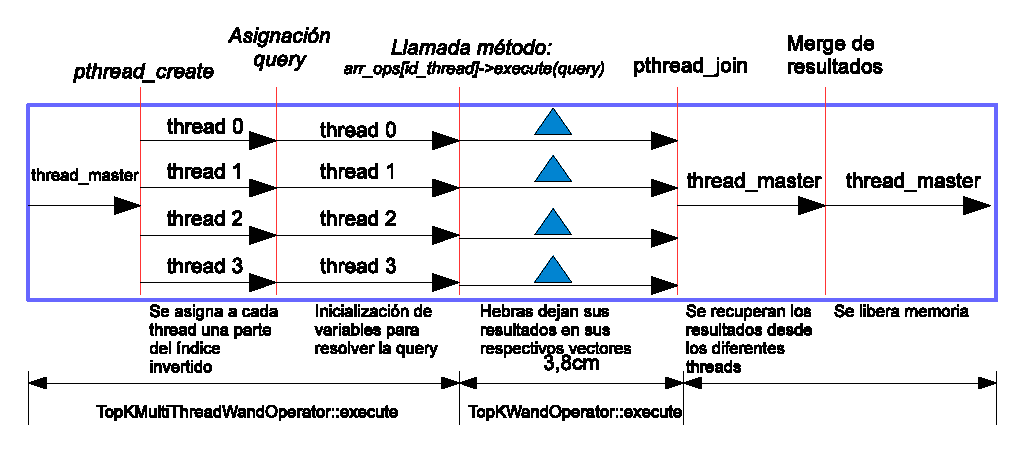
\includegraphics[scale=.75]{images/ejecucion_wandlh.eps}
\caption{Ejemplo de ejecución esquema Wand LH}
\label{fig:ejecucion_wandlh}
\end{figure}

  

%El hecho que en el esquema de heap locales no se requiere mecanismos de control de paralelismo en su implementación, posee ventajas para queries cortas en su procesamiento 
%Figura




\lstinputlisting[label=code:topkmultithreadwandoperatorlocal, caption=Implementación de la clase TopKMultithreadWandOperatorLocal.h, language=C++]{code/TopKMultithreadWandOperatorLocal.h}

Mostrar topK Wand operator



\subsection{Wand heap compartido}
\label{evaluacionexperimental:whc}

 el proceso de descarte tiende a ser más eficiente porque los documentos con mayor puntaje tienden a estar en el heap

Se habla un poco de las ventajas que se tenía con este esquema nuevamente, qué se hizo para la implementación, cómo se programó, etc. 

Se muestra el código y ojalá se muestra algún flujo de ejecución para una query específica.

%\lstinputlisting[language=C++]{code/TopKMultithreadWandOperatorLocal.h}

Se muestra un gráfico y tabla de eficiencia.


\begin{figure}[!ht]
\centering
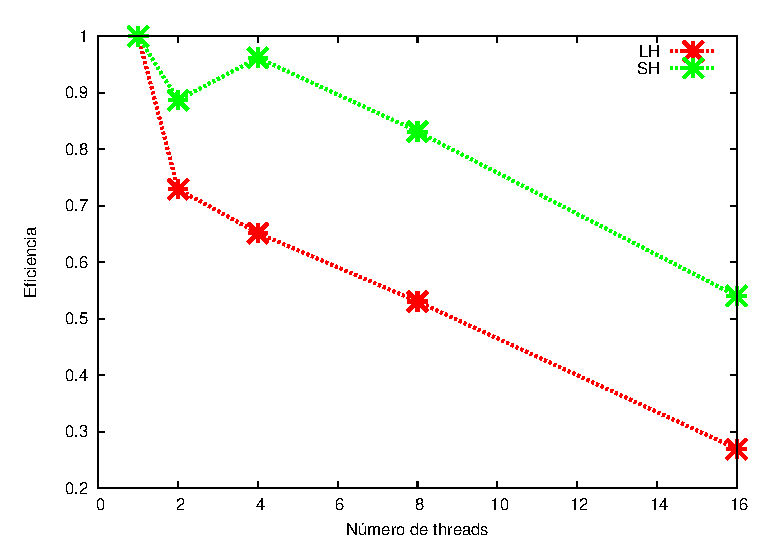
\includegraphics[scale=.75]{images/eficiencias_wand.eps}
\caption{Eficiencias para Wand con heaps compartido y locales}
\label{fig:eficiencias_wand}
\end{figure}


\begin{figure}[!ht]
\centering
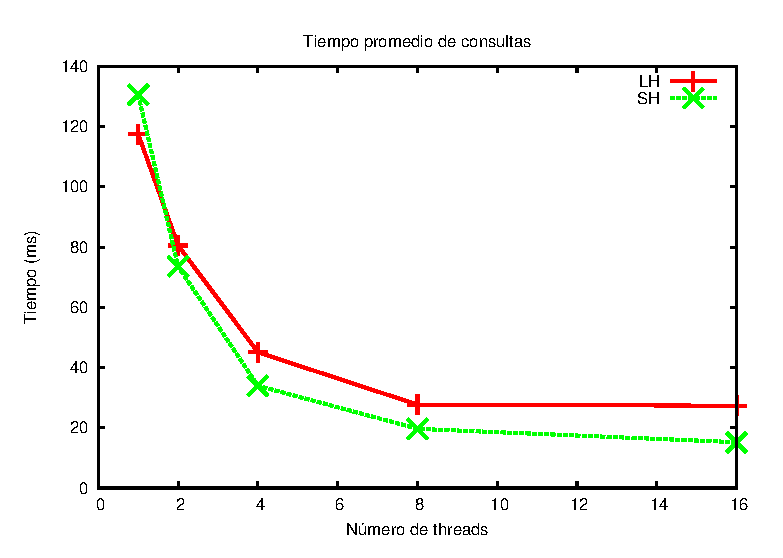
\includegraphics[scale=.75]{images/tiempos_wand.eps}
\caption{Tiempos promedios de las consultas}
\label{fig:tiempos_wand}
\end{figure}

\subsection{Resultados obtenidos}
\label{evaluacionexperimental:resultadosObtenidos}




\section{Estrategias de scheduling}
\label{evaluacionexperimental:estrategiasscheduling}

Hablar separado cada una de ellas, mostrando implementación y cómo se llevaron a cabo los experimentos.

1. Comparar las tres estrategias de scheduling (decir que TimesRanges es mejor) ==> Con predictor perfecto también?
2. Comparar TimesRanges con baseline ==> Con Predictor perfecto también.  
4. Decir los problemas que existen en cada una de las estrategias que se pierden tiempos.
3. Sacar a la luz la nueva unidades de trabajo ==> Predictor perfecto también.
4. Comparación unidades de trabajo - baseline - TimesRanges.

Conclusiones para cada uno de los gráficos realizados. 

Se intuye que habrá pérdida de eficiencia al final de cada bloque en FR.
